\documentclass[12pt,a4paper]{article}
\usepackage[utf8]{inputenc}
\usepackage[english]{babel}
\usepackage{listings}
\usepackage{xcolor}
\usepackage{graphicx}
\usepackage{geometry}
 \geometry{
 a4paper,
 total={170mm,257mm},
 left=25mm,
 top=20mm,
 right=25mm,
 bottom=20mm
 }

\title{\bf BCD to ASCII conversion using 8051}
\author{\vspace{-10ex}}
\date{\vspace{-10ex}}
\begin{document}
\maketitle

\begin{minipage}{0.45\textwidth}
        \begin{tabular}{l l}
            \textbf{Expt No:}&14\\
            \textbf{Date :}&23/10/2020
        \end{tabular}
\end{minipage}%
\begin{minipage}{0.45\textwidth}
        \begin{tabular}{l l}
             \textbf{Name:}& Shivanirudh S G  \\
             \textbf{Reg No:} & 185001146 
        \end{tabular}
\end{minipage}
\vspace{1cm}
\hrule
\begin{flushleft}
\subsection*{\textbf{Aim:}} 
To convert a number from BCD to ASCII using \textbf{8051 microcontroller}.

\subsubsection*{\textbf{Algorithm:}}
\begin{itemize}
    \item Move hex value 00 to register 0. 
    \item Move the value of register 1 to A.
    \item Mask upper bits of A using ANL A, 0FH.
    \item Add hex value 30 using ADD A, 30H to convert it to ASCII.
    \item Store converted lower bits in Register 5.
    \item Move value of register 1 to A.
    \item Mask lower bits of A using ANL A, 0F0H.
    \item Swap upper and lower nibbles using SWAP A.
    \item Add hex value 30 using ADD A, 30H to convert it to ASCII.
    \item Store converted upper bits in Register 4.
\end{itemize}

\newpage
\subsubsection*{\textbf{Program:}}

\begin{table}[htb]
\centering
\begin{tabular}{|l|l|} 
\hline
\textbf{Program}                                                 & \textbf{Comments}                             \\ 
\hline
\hline
mov r0, \#00                                                     & Move hex value 00 to Register 0               \\
\hline
mov a, r1                                                        & Move value in Register 1 to A                 \\
\hline
anl a, \#0FH                                                      & Mask upper bits                              \\
\hline
add a, \#30H                                                      & Add hex value 30 to convert to ASCII         \\
\hline
mov r5, a                                                        & Store converted lower bits into Register 5    \\
\hline
mov a, r1                                                        & Move value in Register 1 to A                 \\
\hline
anl a, \#0F0H                                                     & Mask lower bits                              \\
\hline
swap a                                                           & Swap upper and lower nibbles of A             \\
\hline
add a, \#30H                                                      & Add hex value 30 to convert to ASCII         \\
\hline 
mov r4, a                                                        & Store converted upper bits into Register 4    \\
\hline
here:~sjmp here                                                  & Halt                                          \\
\hline
\end{tabular}
\end{table}

\subsubsection*{\textbf{Input and Output:}}
\begin{figure}[h]
    \centering
    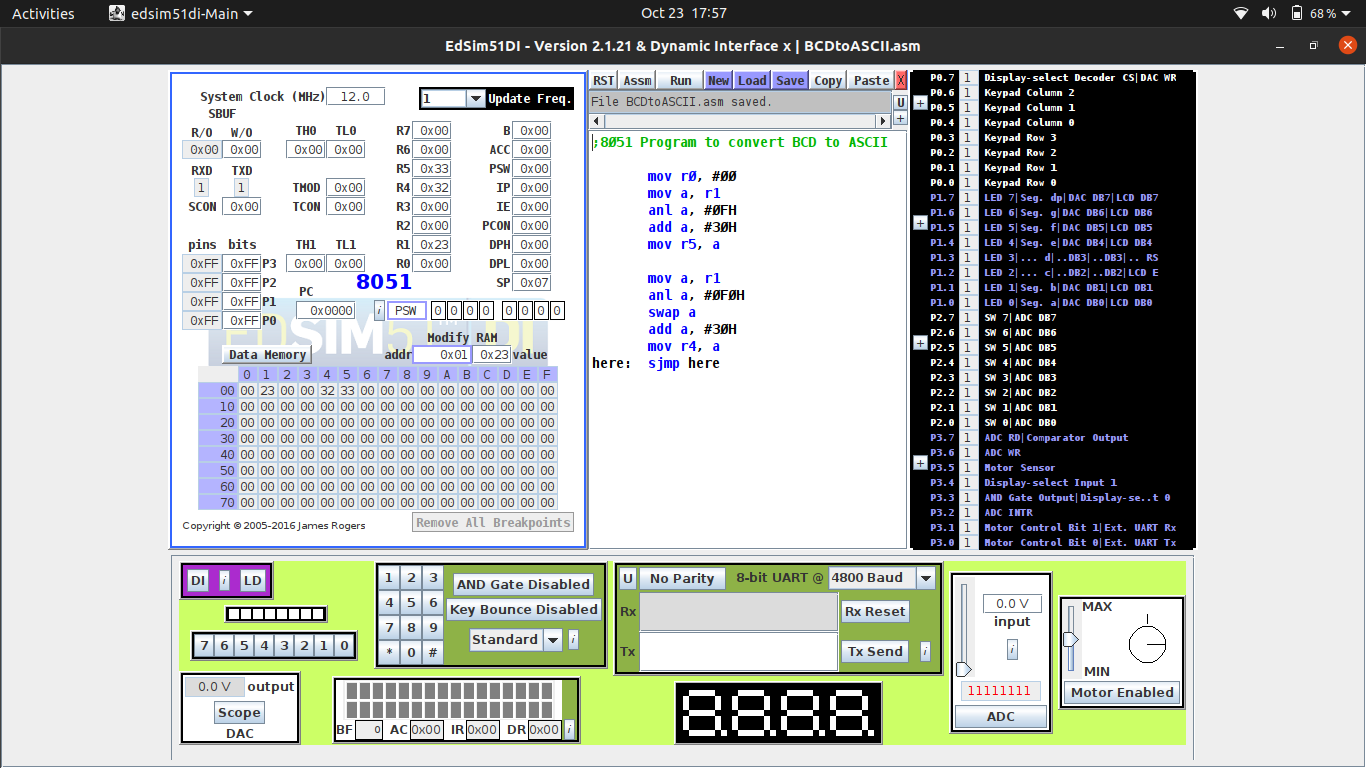
\includegraphics[trim = 60mm 75mm 60mm 10mm, clip, width = \textwidth]{Pics/BCDtoASCII.png}
    \caption{ \textbf{Input:} r1: 23h; 
              \textbf{Output:} Higher: 32h, Lower: 33h}
\end{figure}
\hrule
\subsection*{\textbf{Result:}}
The 8051 program to convert a number from BCD to ASCII was written, and the results observed.
\end{flushleft}
\end{document}